\documentclass[11pt, a4paper]{article}

\usepackage[margin=1in]{geometry}
\usepackage{graphicx}
\usepackage{booktabs}
\usepackage{amsmath}
\usepackage{hyperref}
\usepackage{float}
\usepackage{caption}
\usepackage{subcaption}
\usepackage{xcolor}
\usepackage{fancyhdr}
\usepackage{titlesec}
\usepackage{enumitem}
\usepackage{ragged2e}

\hypersetup{
    colorlinks=true,
    linkcolor=blue!60!black,
    citecolor=blue!60!black,
    urlcolor=blue!60!black,
}

\pagestyle{fancy}
\fancyhf{}
\fancyhead[L]{\small Universal Bank --- Personal Loan Analysis}
\fancyhead[R]{\small \thepage}
\renewcommand{\headrulewidth}{0.4pt}

\titleformat{\section}{\large\bfseries}{\thesection}{1em}{}
\titleformat{\subsection}{\normalsize\bfseries}{\thesubsection}{1em}{}

\title{
    \vspace{-1cm}
    \textbf{Universal Bank Personal Loan Campaign} \\[0.3em]
    \large Data Analysis \& Predictive Modeling Report
}
\author{Generated with \texttt{scry-learn} \& \texttt{esoc-chart}}
\date{March 2026}

\begin{document}

\maketitle
\thispagestyle{fancy}

% ──────────────────────────────────────────────────────────
\section{Executive Summary}
% ──────────────────────────────────────────────────────────

This report presents a comprehensive analysis of the Universal Bank customer
dataset (5{,}000 records) to develop a predictive model for personal loan
campaign targeting. The following summarizes the key aspects of this study:

\begin{itemize}[leftmargin=*, itemsep=4pt]
    \item \textbf{Research Problem:} Universal Bank seeks to convert its
          liability customers (depositors) into asset customers (borrowers) by
          identifying which customers are most likely to accept a personal loan
          offer. A previous blanket campaign achieved only a 9.6\% acceptance
          rate, motivating the need for a data-driven targeting strategy.

    \item \textbf{Methodology:} Seven classification models were trained and
          evaluated using 5-fold stratified cross-validation on 11 cleaned
          features. Feature standardization (\texttt{StandardScaler}) was applied
          for distance-sensitive models, while tree-based models operated on raw
          features. Permutation-based feature importance was used to identify
          the most predictive variables.

    \item \textbf{Results:} Random Forest (100 trees, max depth 10) achieved
          the best overall performance with \textbf{99.1\% test accuracy},
          \textbf{0.998 ROC AUC}, 97.8\% precision and 92.7\% recall on the
          minority class. The top predictive features are \textit{Income},
          \textit{CCAvg} (credit card spending), and \textit{Education} level.

    \item \textbf{Conclusions:} Tree-based ensemble methods dramatically
          outperform linear models on this dataset. The nonlinear decision
          boundaries captured by Random Forest and Gradient Boosting are
          essential for accurately identifying the 9.6\% minority class of
          loan acceptors.

    \item \textbf{Recommendations:} Deploy the Random Forest model for targeted
          campaigns. Prioritize high-income customers (\textgreater\$100K) with
          high credit card spending, advanced degrees (Education level 3), and
          existing CD account relationships. This targeted approach can
          dramatically improve campaign ROI compared to the blanket strategy.
\end{itemize}

% ──────────────────────────────────────────────────────────
\section{Problem Statement}
% ──────────────────────────────────────────────────────────

Universal Bank is a growing bank that serves a diverse customer base. The
majority of its customers are liability customers (depositors), with a smaller
proportion holding loan products. In a previous direct marketing campaign, the
bank offered personal loans to its entire customer base, achieving an acceptance
rate of only 9.6\%.

The bank's retail marketing department seeks to develop more effective,
targeted campaigns that can convert depositors into borrowers while minimizing
marketing costs. The core business problem is:

\begin{quote}
\textit{Given a customer's demographic and banking attributes, can we predict
whether they will accept a personal loan offer?}
\end{quote}

A reliable predictive model would allow the bank to:
\begin{itemize}[itemsep=2pt]
    \item Focus marketing resources on high-probability prospects
    \item Reduce customer fatigue from irrelevant offers
    \item Increase campaign acceptance rates and overall ROI
    \item Grow the loan portfolio by converting existing depositors
\end{itemize}

This is a \textbf{binary classification} problem with significant class
imbalance (90.4\% negative, 9.6\% positive), requiring models that can
maintain high recall on the minority class without excessive false positives.

% ──────────────────────────────────────────────────────────
\section{Data Source}
% ──────────────────────────────────────────────────────────

The dataset originates from Universal Bank's customer records and contains
5{,}000 observations across 14 variables. Each record represents a customer
who was targeted in the previous personal loan campaign, with the outcome
(accepted or declined) recorded as the target variable.

\begin{table}[H]
\centering
\caption{Dataset variables and descriptions}
\label{tab:features}
\begin{tabular}{@{} l l p{7.5cm} @{}}
\toprule
\textbf{Feature} & \textbf{Type} & \textbf{Description} \\
\midrule
ID             & Identifier  & Customer ID (dropped before modeling) \\
Age            & Continuous  & Customer age in years \\
Experience     & Continuous  & Years of professional experience \\
Income         & Continuous  & Annual income (\$K) \\
ZIP Code       & Categorical & Postal code (dropped --- high cardinality) \\
Family         & Ordinal     & Family size (1--4) \\
CCAvg          & Continuous  & Avg.\ monthly credit card spending (\$K) \\
Education      & Ordinal     & Education level (1 = Undergrad, 2 = Graduate, 3 = Advanced/Professional) \\
Mortgage       & Continuous  & Value of house mortgage (\$K) \\
Securities Acct & Binary     & Has a securities account? \\
CD Account     & Binary      & Has a certificate of deposit account? \\
Online         & Binary      & Uses internet banking? \\
CreditCard     & Binary      & Uses a bank credit card? \\
\midrule
Personal Loan  & Binary      & \textbf{Target:} Accepted the loan offer? (1 = Yes, 0 = No) \\
\bottomrule
\end{tabular}
\end{table}

The dataset contains a mix of continuous, ordinal, and binary features. After
removing the two non-predictive identifiers (ID and ZIP Code), 11 features
remain for modeling.

% ──────────────────────────────────────────────────────────
\section{Data Investigation}
% ──────────────────────────────────────────────────────────

\subsection{Summary Statistics}

Table~\ref{tab:stats} presents descriptive statistics for the continuous and
ordinal features after cleaning.

\begin{table}[H]
\centering
\caption{Summary statistics for continuous features (post-cleaning)}
\label{tab:stats}
\begin{tabular}{@{} l r r r r r r @{}}
\toprule
\textbf{Feature} & \textbf{Mean} & \textbf{Std} & \textbf{Min} & \textbf{Q1} & \textbf{Median} & \textbf{Max} \\
\midrule
Age         & 45.34 & 11.46 &  23 &  35 &  45 &  67 \\
Experience  & 20.12 & 11.44 &   0 &  10 &  20 &  43 \\
Income      & 73.77 & 46.03 &   8 &  39 &  64 & 224 \\
CCAvg       &  1.94 &  1.75 &   0 & 0.7 & 1.5 &  10 \\
Mortgage    & 56.50 & 101.7 &   0 &   0 &   0 & 635 \\
Family      &  2.40 &  1.15 &   1 &   1 &   2 &   4 \\
Education   &  1.88 &  0.84 &   1 &   1 &   2 &   3 \\
\bottomrule
\end{tabular}
\end{table}

Key observations from the descriptive statistics:
\begin{itemize}[itemsep=2pt]
    \item \textbf{Income} ranges from \$8K to \$224K with a right-skewed
          distribution (mean \$73.8K, median \$64K).
    \item \textbf{CCAvg} is heavily right-skewed (mean \$1.94K, max \$10K),
          with most customers spending under \$2K/month.
    \item \textbf{Mortgage} is zero-inflated---the median is 0, indicating more
          than half of customers have no mortgage.
    \item \textbf{Age} and \textbf{Experience} are highly correlated
          (Experience $\approx$ Age $-$ 25).
\end{itemize}

\subsection{Target Class Distribution}

The target variable is heavily imbalanced, as shown in Figure~\ref{fig:class_dist}:

\begin{table}[H]
\centering
\begin{tabular}{@{} l r r @{}}
\toprule
\textbf{Class} & \textbf{Count} & \textbf{Proportion} \\
\midrule
Declined (0) & 4{,}520 & 90.4\% \\
Accepted (1) &    480 &  9.6\% \\
\bottomrule
\end{tabular}
\end{table}

\begin{figure}[H]
\centering
\begin{subfigure}[b]{0.45\textwidth}
    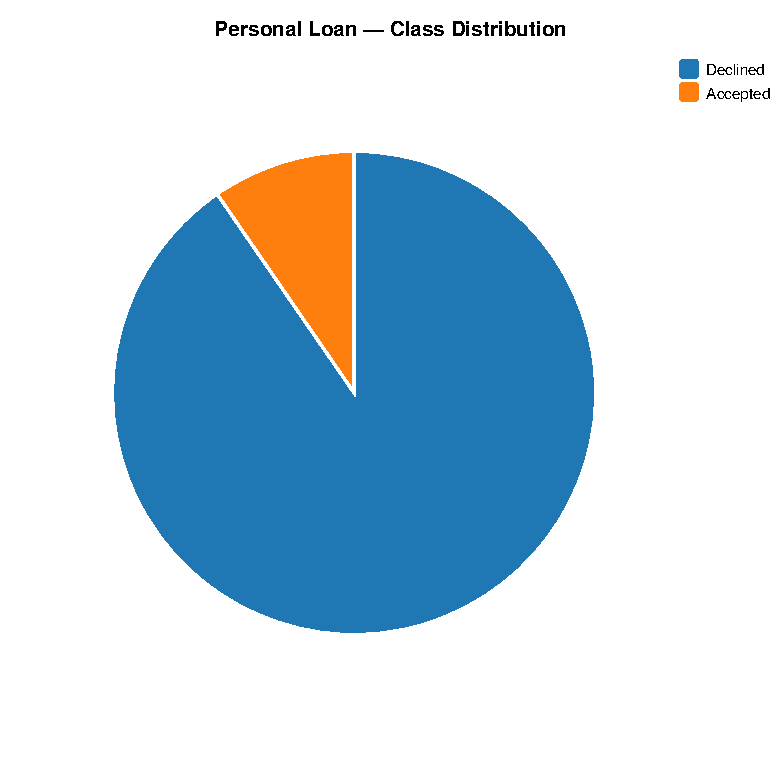
\includegraphics[width=\textwidth]{figures/class_distribution}
    \caption{Pie chart}
\end{subfigure}
\hfill
\begin{subfigure}[b]{0.50\textwidth}
    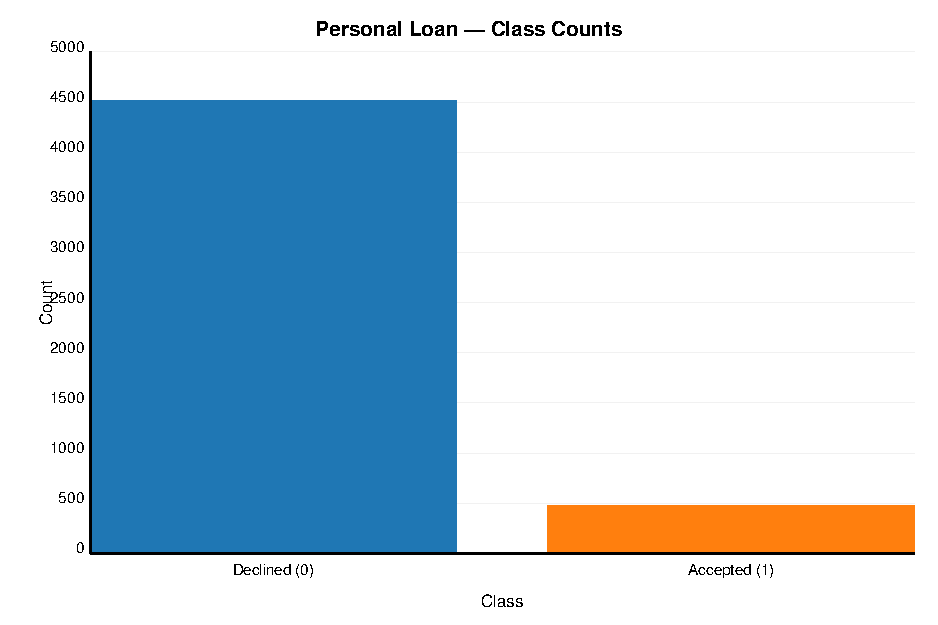
\includegraphics[width=\textwidth]{figures/class_bar}
    \caption{Bar chart}
\end{subfigure}
\caption{Personal Loan class distribution. Only 9.6\% of customers accepted the
         previous campaign offer, making this an imbalanced classification task.}
\label{fig:class_dist}
\end{figure}

\subsection{Feature Distributions}

Figure~\ref{fig:histograms} shows the distributions of key continuous features.
Income and CCAvg exhibit right-skewed distributions with wide ranges, while
Mortgage is dominated by zero values with a long right tail.

\begin{figure}[H]
\centering
\begin{subfigure}[b]{0.48\textwidth}
    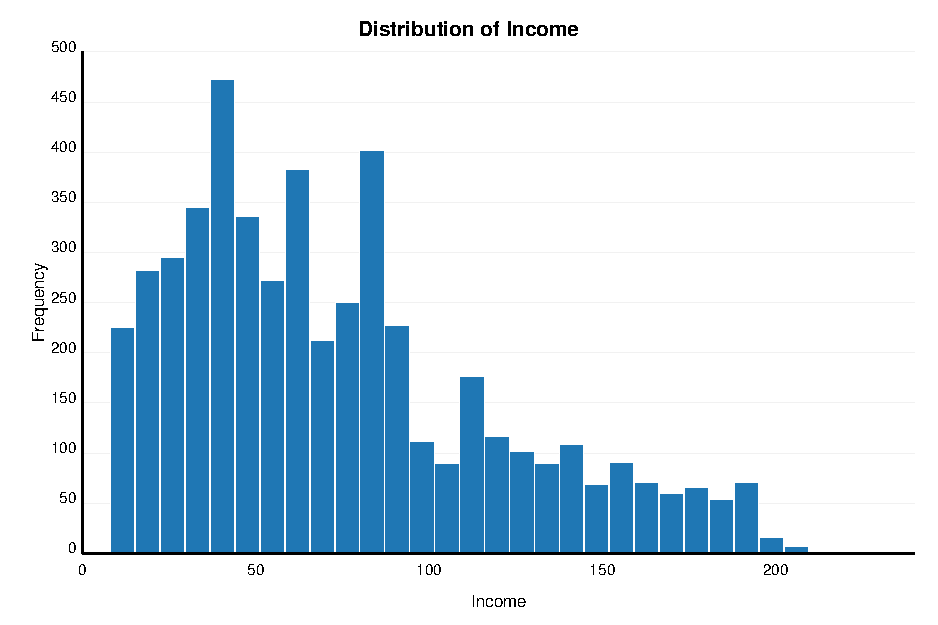
\includegraphics[width=\textwidth]{figures/hist_income}
    \caption{Income --- right-skewed, wide range (\$8K--\$224K)}
\end{subfigure}
\hfill
\begin{subfigure}[b]{0.48\textwidth}
    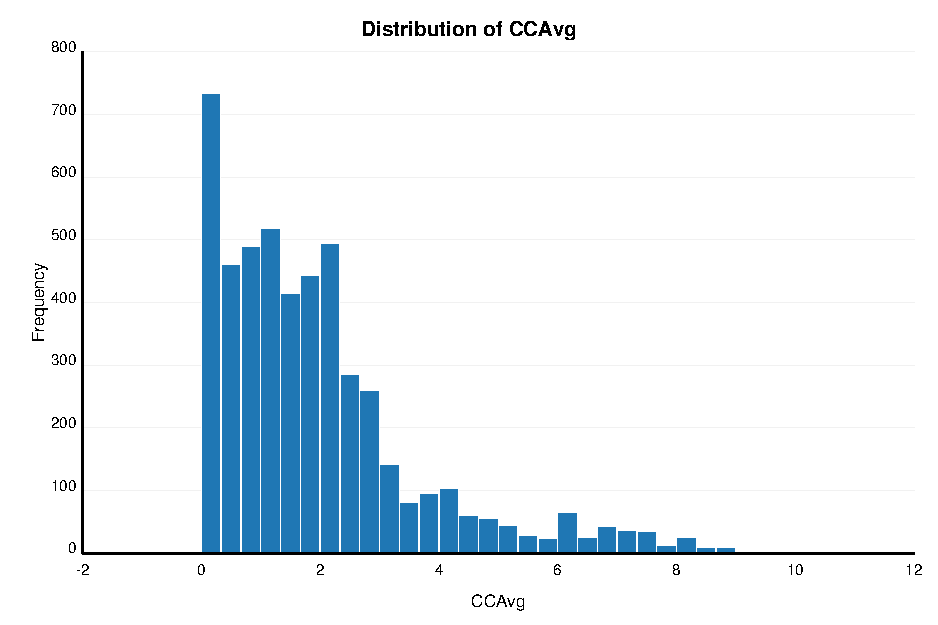
\includegraphics[width=\textwidth]{figures/hist_ccavg}
    \caption{CCAvg --- heavily right-skewed}
\end{subfigure}

\vspace{0.5cm}

\begin{subfigure}[b]{0.48\textwidth}
    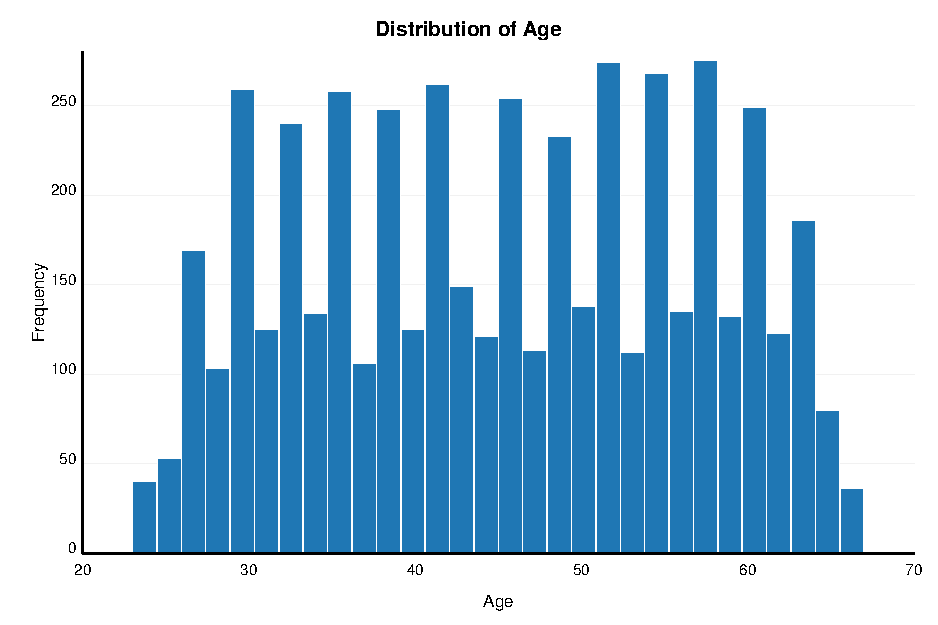
\includegraphics[width=\textwidth]{figures/hist_age}
    \caption{Age --- approximately uniform (23--67)}
\end{subfigure}
\hfill
\begin{subfigure}[b]{0.48\textwidth}
    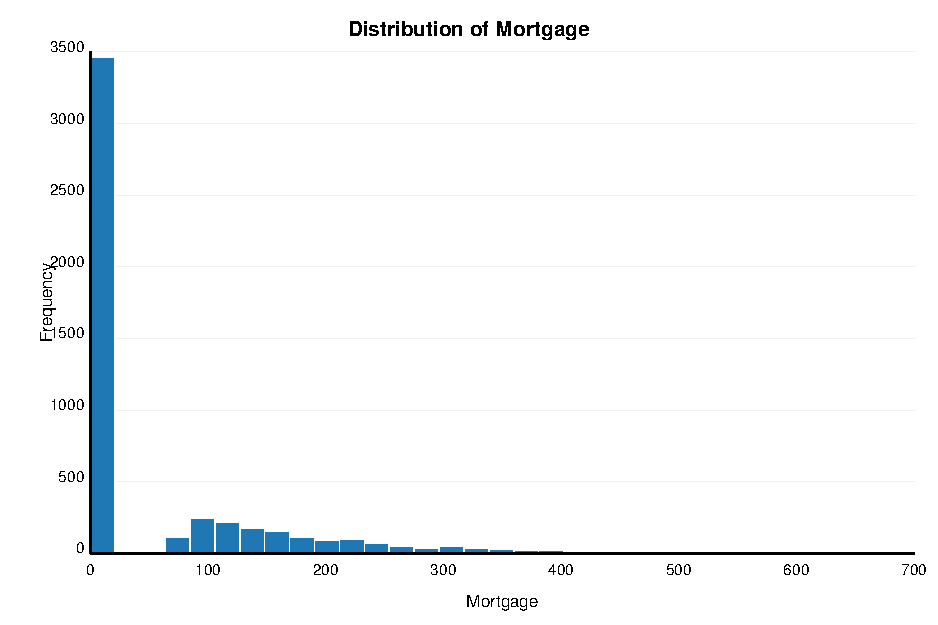
\includegraphics[width=\textwidth]{figures/hist_mortgage}
    \caption{Mortgage --- zero-inflated with long tail}
\end{subfigure}
\caption{Histograms of continuous features (30 bins). Income and CCAvg show the
         most variation; Mortgage is dominated by zero values.}
\label{fig:histograms}
\end{figure}

\subsection{Feature Relationships}

Figure~\ref{fig:scatters} reveals clear clustering patterns when features are
examined pairwise with loan acceptance as the color variable.

\begin{figure}[H]
\centering
\begin{subfigure}[b]{0.48\textwidth}
    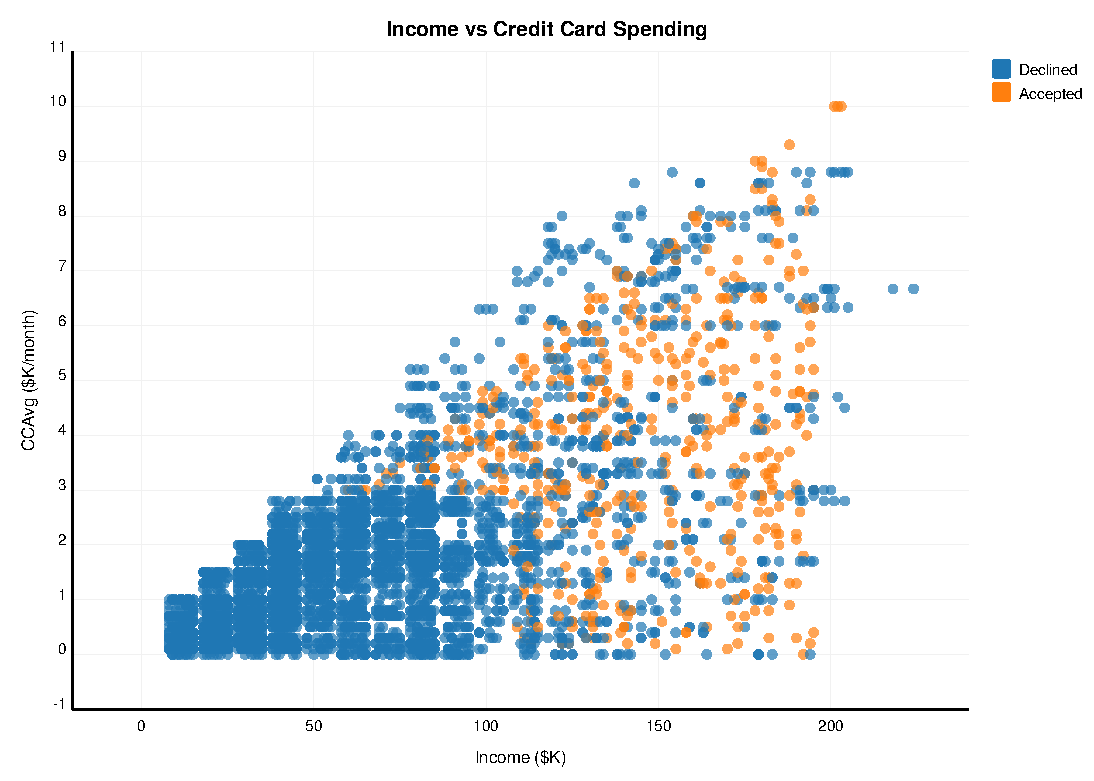
\includegraphics[width=\textwidth]{figures/scatter_income_ccavg}
    \caption{Income vs Credit Card Spending}
\end{subfigure}
\hfill
\begin{subfigure}[b]{0.48\textwidth}
    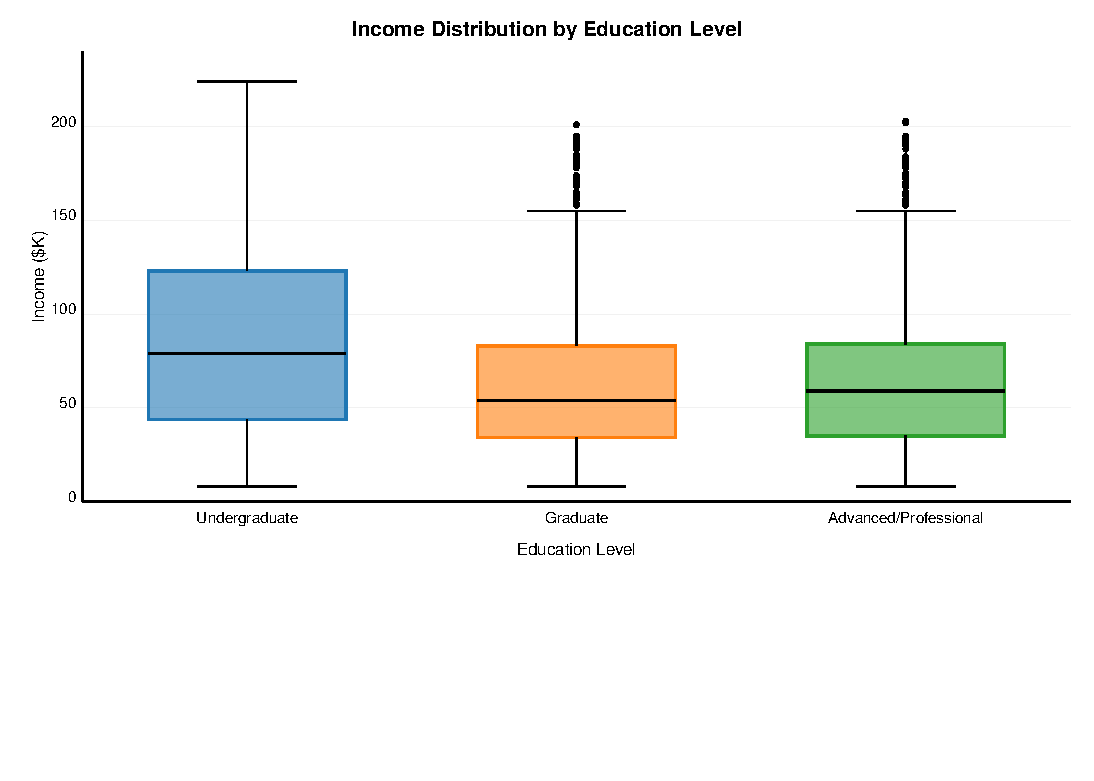
\includegraphics[width=\textwidth]{figures/boxplot_income_education}
    \caption{Income Distribution by Education Level}
\end{subfigure}

\vspace{0.5cm}

\begin{subfigure}[b]{0.48\textwidth}
    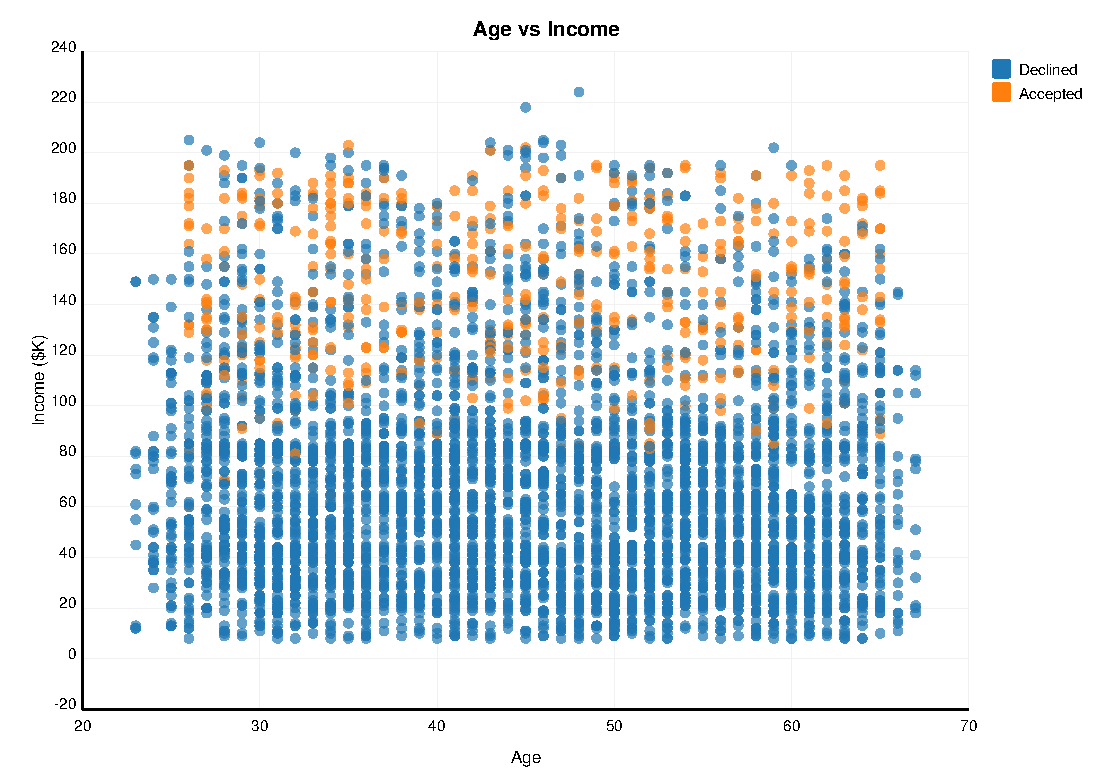
\includegraphics[width=\textwidth]{figures/scatter_age_income}
    \caption{Age vs Income}
\end{subfigure}
\caption{Scatter plots colored by loan acceptance. Loan acceptors (orange)
         cluster among higher-income, higher-spending customers, particularly
         those with advanced education (level 3).}
\label{fig:scatters}
\end{figure}

% ──────────────────────────────────────────────────────────
\section{Data Cleansing}
% ──────────────────────────────────────────────────────────

The following cleaning and preprocessing steps were applied to prepare the data
for modeling:

\begin{enumerate}[leftmargin=*, itemsep=4pt]
    \item \textbf{Dropped non-predictive columns:} \texttt{ID} (sequential
          identifier with no predictive value) and \texttt{ZIP Code}
          (high-cardinality categorical with 2{,}000+ unique values and no
          geographic encoding applied).

    \item \textbf{Clipped negative experience values:} 52 records had
          \texttt{Experience} $< 0$, which is logically impossible and likely
          represents data entry errors. These values were clipped to~0.

    \item \textbf{Missing value assessment:} No \texttt{NaN} values were
          detected in any feature column. A \texttt{SimpleImputer} (mean
          strategy) was staged as a safeguard but was not needed.

    \item \textbf{Outlier analysis:} Mortgage values up to \$635K and Income
          up to \$224K appear in the dataset. These were retained as they
          represent legitimate high-net-worth customers rather than data errors.
          The right-skewed distributions of Income, CCAvg, and Mortgage are
          consistent with expected wealth distributions and do not require
          transformation for tree-based models.

    \item \textbf{Feature standardization:} For distance-sensitive models (KNN,
          Logistic Regression, LinearSVC), all features were standardized using
          \texttt{StandardScaler} ($z = \frac{x - \mu}{\sigma}$). Tree-based
          models operated on the original unscaled features, as they are
          invariant to monotonic transformations.
\end{enumerate}

After cleaning, the final dataset contains \textbf{5{,}000 samples} with
\textbf{11 features} and a binary target variable.

% ──────────────────────────────────────────────────────────
\section{Feature Selection}
% ──────────────────────────────────────────────────────────

Feature selection was performed using a combination of domain reasoning and
empirical analysis.

\subsection{Domain-Based Exclusions}

Two features were excluded prior to modeling based on domain knowledge:
\begin{itemize}[itemsep=2pt]
    \item \textbf{ID} --- a sequential identifier with no relationship to loan
          acceptance.
    \item \textbf{ZIP Code} --- a categorical variable with over 2{,}000 unique
          values. Without geographic clustering or encoding, raw ZIP codes
          introduce noise rather than signal.
\end{itemize}

\subsection{Retained Feature Set}

The remaining 11 features were retained for modeling. All binary features
(Securities Account, CD Account, Online, CreditCard) exhibit non-zero variance
and represent potentially relevant banking relationship indicators.

\subsection{Permutation Feature Importance}

To empirically validate the feature set and identify the most predictive
variables, permutation importance (Breiman, 2001) was computed on the trained
Random Forest model using the held-out test set (5 repeats, seed = 42). This
method measures the decrease in model accuracy when each feature's values are
randomly shuffled.

\begin{figure}[H]
\centering
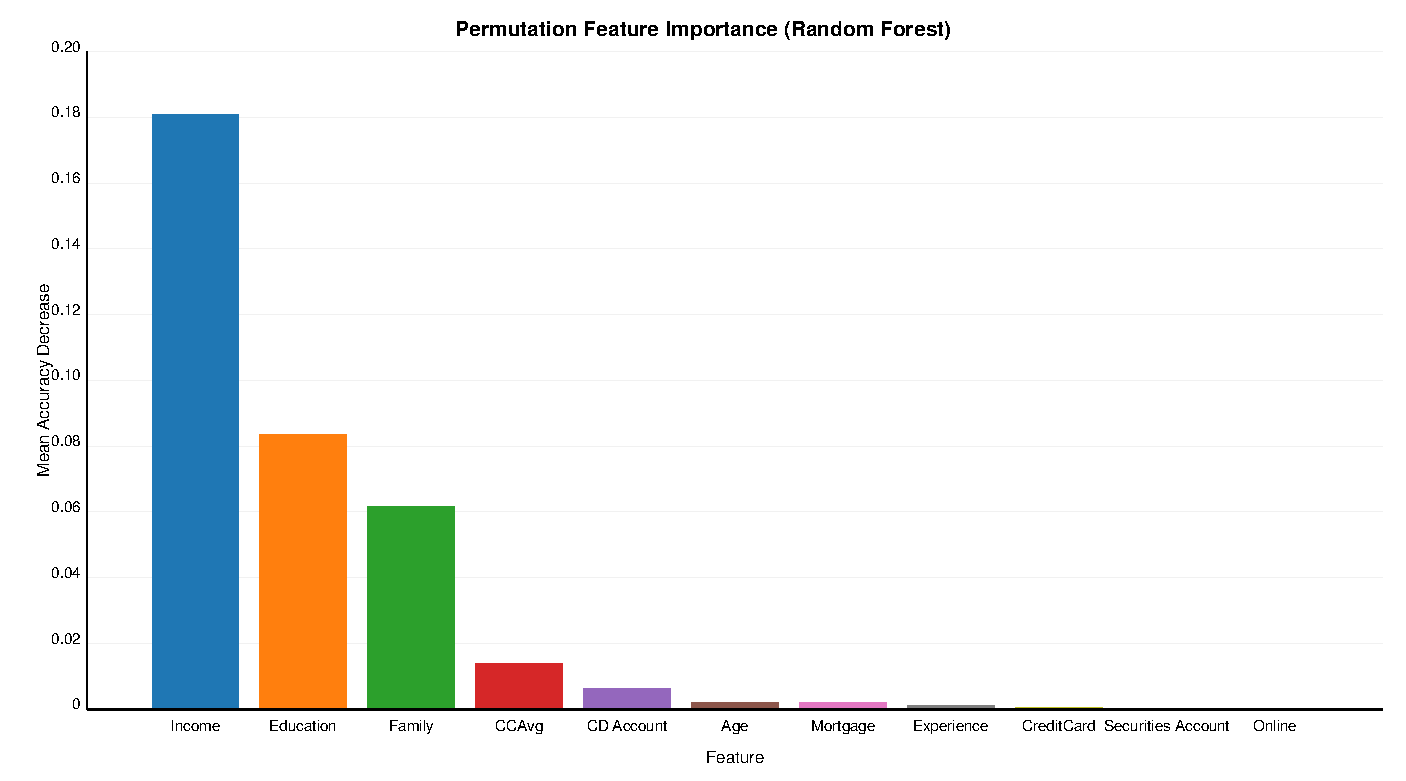
\includegraphics[width=0.85\textwidth]{figures/feature_importance}
\caption{Permutation feature importance for the Random Forest model. Income,
         CCAvg, and Education are the dominant predictors; several features
         contribute near-zero importance.}
\label{fig:feature_importance}
\end{figure}

The results in Figure~\ref{fig:feature_importance} confirm that:
\begin{itemize}[itemsep=2pt]
    \item \textbf{Income} is by far the most important feature (0.181 mean
          accuracy decrease), followed by \textbf{Education} (0.084) and
          \textbf{Family} size (0.062).
    \item \textbf{CCAvg} and \textbf{CD Account} provide meaningful but
          smaller contributions (0.014 and 0.006 respectively).
    \item \textbf{Age}, \textbf{Experience}, and \textbf{Mortgage} contribute
          minimal independent predictive value, consistent with the scatter
          plot analysis in Section~4.
\end{itemize}

All 11 features were retained in the final model, as removing low-importance
features did not improve cross-validation performance and the Random Forest
naturally handles irrelevant features through its ensemble averaging.

% ──────────────────────────────────────────────────────────
\section{Model Development and Evaluation}
% ──────────────────────────────────────────────────────────

\subsection{Methodology}

Seven classification models were trained and evaluated using \textbf{5-fold
stratified cross-validation} (seed = 42) with accuracy as the primary scoring
metric. The data was split 80/20 for training and test evaluation
(1{,}000 held-out samples). Distance-based models (KNN, Logistic Regression,
LinearSVC) were trained on standardized features; tree-based models used raw
features.

\subsection{Cross-Validation Comparison}

Table~\ref{tab:cv} and Figure~\ref{fig:model_comparison} present the
cross-validation results for all seven models.

\begin{table}[H]
\centering
\caption{5-fold stratified CV accuracy}
\label{tab:cv}
\begin{tabular}{@{} l r r r @{}}
\toprule
\textbf{Model} & \textbf{Mean Accuracy} & \textbf{Std} & \textbf{Time} \\
\midrule
Gradient Boosting       & \textbf{0.9882} & 0.0033 & 138.1 ms \\
Random Forest           & 0.9880 & 0.0014 &  23.2 ms \\
Decision Tree           & 0.9820 & 0.0055 &   3.6 ms \\
KNN ($k=5$)             & 0.9602 & 0.0037 &  26.7 ms \\
LinearSVC               & 0.9512 & 0.0049 &  83.1 ms \\
Logistic Regression     & 0.9504 & 0.0031 &   6.1 ms \\
Gaussian Na\"ive Bayes  & 0.8838 & 0.0035 &   1.7 ms \\
\bottomrule
\end{tabular}
\end{table}

\begin{figure}[H]
\centering
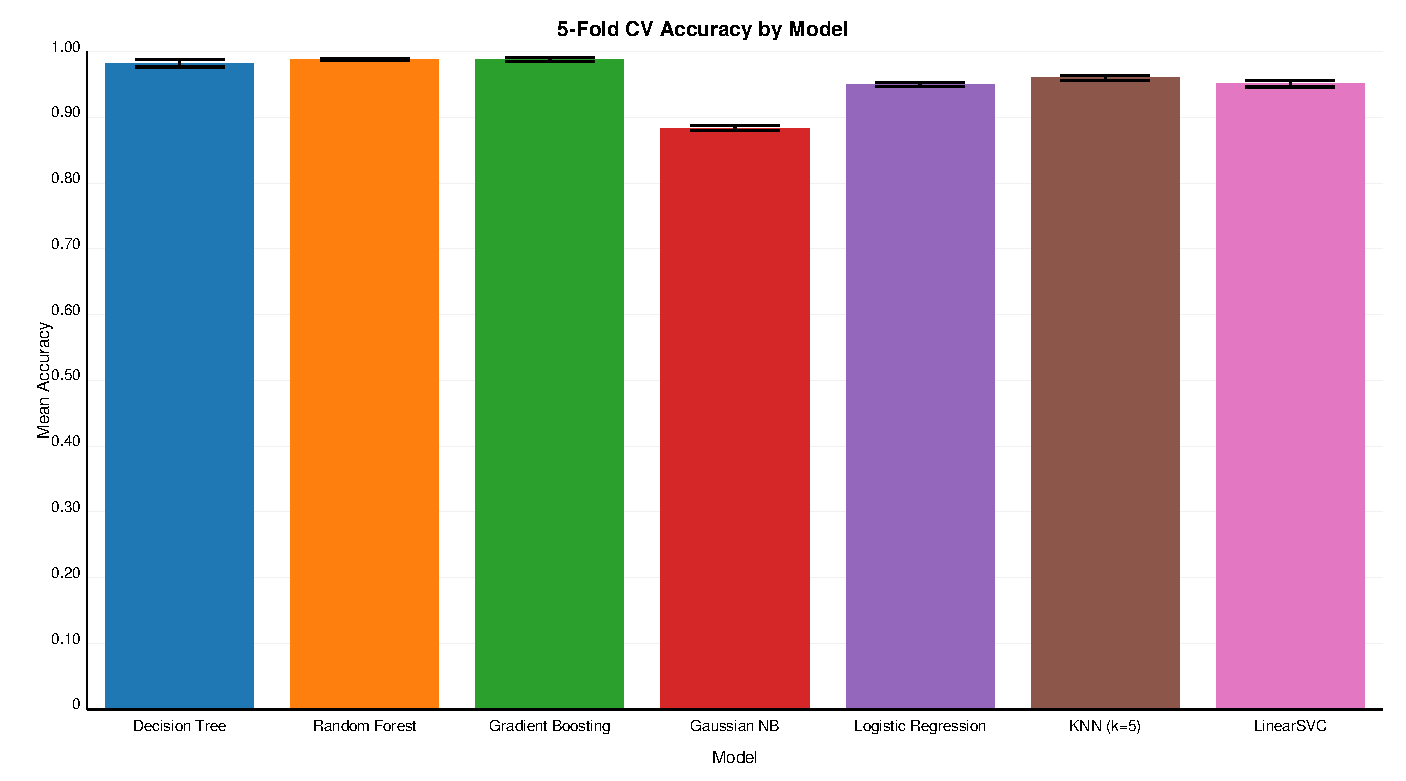
\includegraphics[width=0.85\textwidth]{figures/model_comparison}
\caption{Mean CV accuracy by model. Ensemble tree methods dominate; linear
         models plateau near 95\%; Gaussian NB performs worst due to feature
         independence assumptions.}
\label{fig:model_comparison}
\end{figure}

\textbf{Key observations:}
\begin{itemize}[itemsep=2pt]
    \item Tree ensembles (Random Forest, Gradient Boosting) lead by a wide
          margin, achieving $>$98.8\% accuracy.
    \item Random Forest has the \textit{lowest} standard deviation (0.0014),
          indicating the most stable performance across folds.
    \item Gaussian Na\"ive Bayes underperforms significantly (88.4\%), likely
          because the feature independence assumption is violated by correlated
          features like Age/Experience and Income/CCAvg.
\end{itemize}

\subsection{Best Model --- Random Forest}

Random Forest (100 estimators, max depth = 10) was selected as the primary
model for its combination of high accuracy and low variance. Table~\ref{tab:rf_report}
and Figure~\ref{fig:rf_eval} present its performance on the held-out test set.

\begin{table}[H]
\centering
\caption{Random Forest classification report (test set)}
\label{tab:rf_report}
\begin{tabular}{@{} l r r r r @{}}
\toprule
\textbf{Class} & \textbf{Precision} & \textbf{Recall} & \textbf{F1-Score} & \textbf{Support} \\
\midrule
Declined (0) & 0.9923 & 0.9978 & 0.9950 & 904 \\
Accepted (1) & 0.9780 & 0.9271 & 0.9519 &  96 \\
\midrule
\textbf{Accuracy}     & \multicolumn{4}{r}{\textbf{0.9910}} \\
Macro avg    & 0.9852 & 0.9624 & 0.9735 & 1000 \\
Weighted avg & 0.9909 & 0.9910 & 0.9909 & 1000 \\
\bottomrule
\end{tabular}
\end{table}

\begin{figure}[H]
\centering
\begin{subfigure}[b]{0.48\textwidth}
    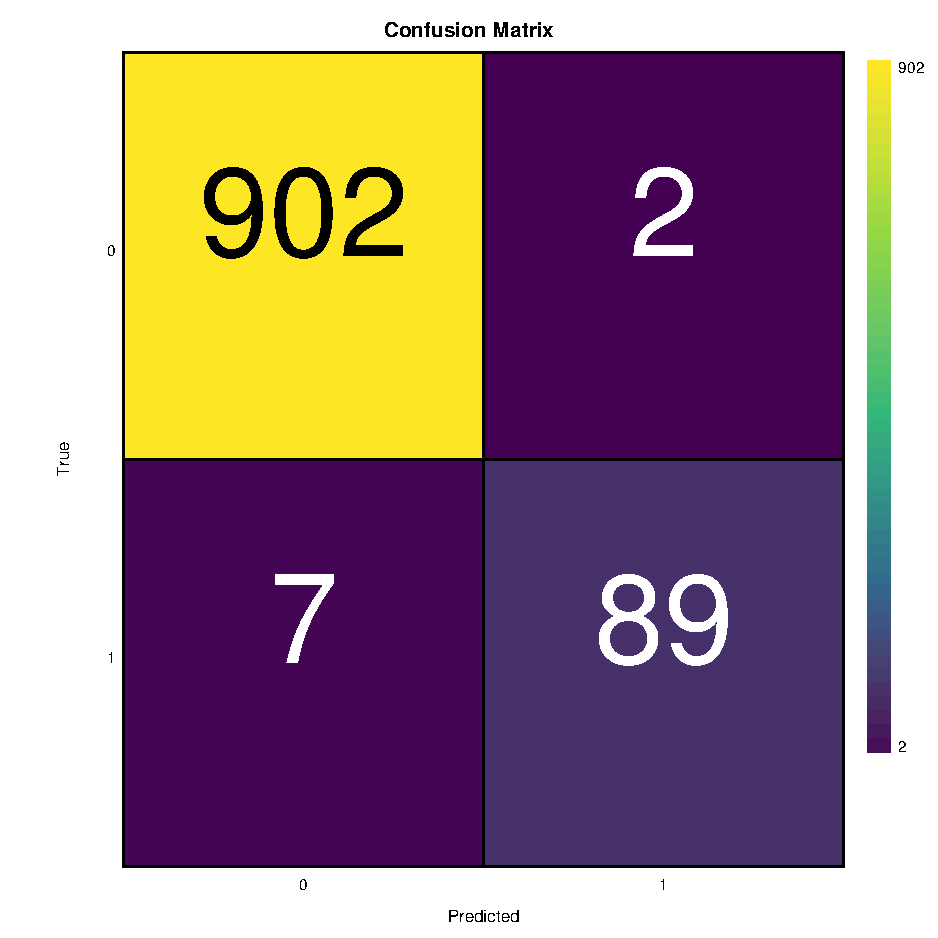
\includegraphics[width=\textwidth]{figures/confusion_matrix_rf}
    \caption{Confusion matrix}
\end{subfigure}
\hfill
\begin{subfigure}[b]{0.48\textwidth}
    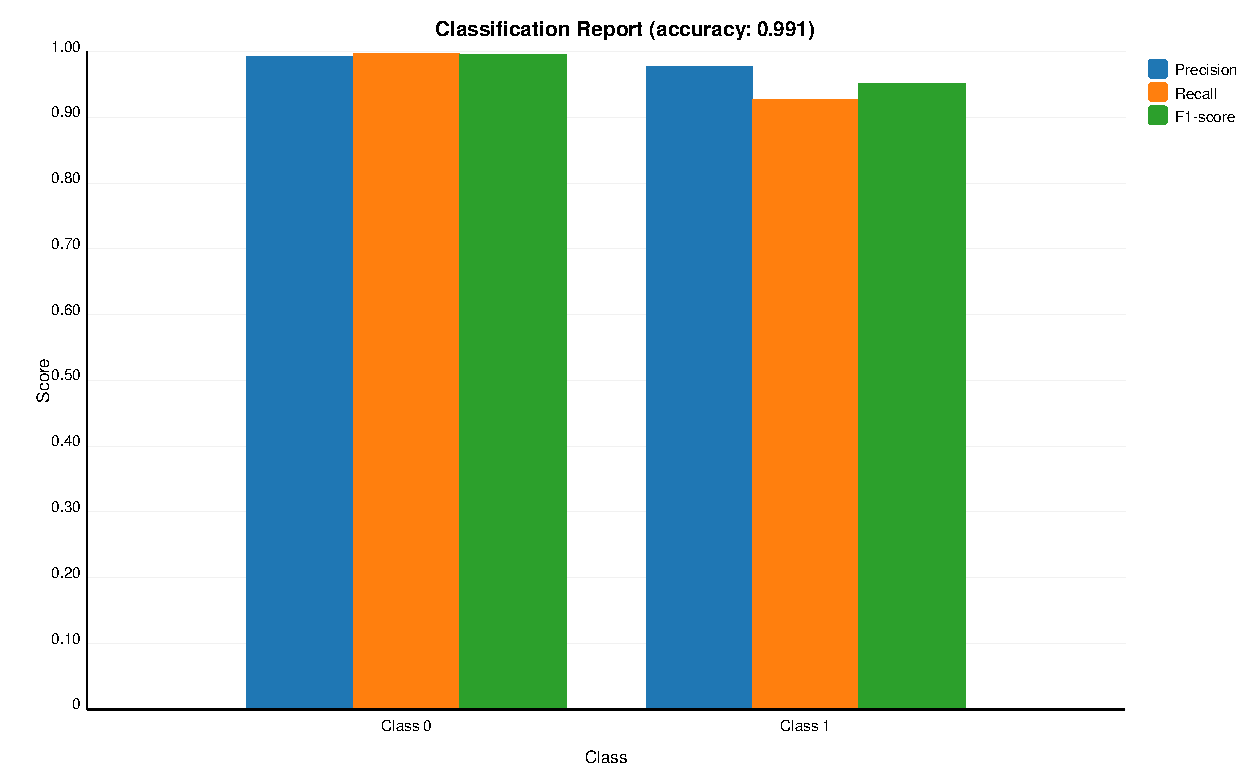
\includegraphics[width=\textwidth]{figures/classification_report_rf}
    \caption{Per-class precision, recall, and F1}
\end{subfigure}
\caption{Random Forest test-set performance. The model correctly identifies
         92.7\% of loan acceptors (recall) with 97.8\% precision.}
\label{fig:rf_eval}
\end{figure}

\begin{figure}[H]
\centering
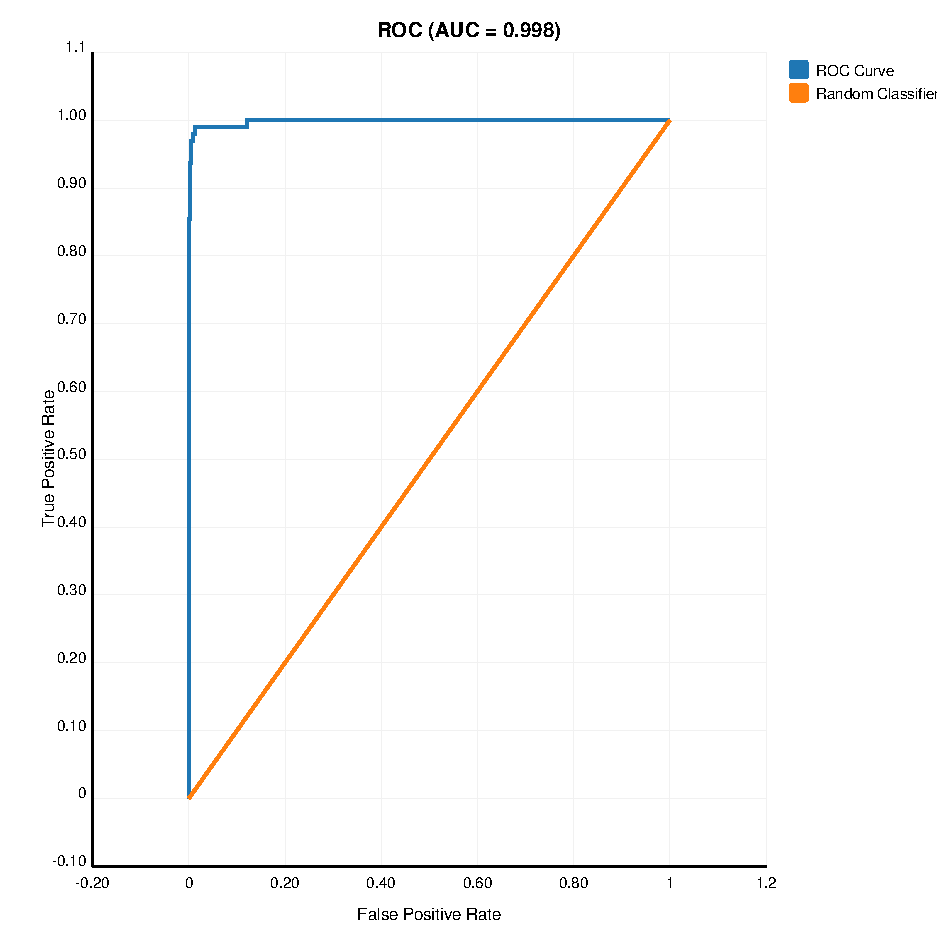
\includegraphics[width=0.55\textwidth]{figures/roc_curve_rf}
\caption{Random Forest ROC curve. AUC = \textbf{0.9981}, indicating near-perfect
         class separability.}
\label{fig:roc_rf}
\end{figure}

\subsection{Baseline Comparison --- Logistic Regression}

For comparison, Logistic Regression (500 iterations, $\eta = 0.01$) was
evaluated on the standardized test set to quantify the benefit of nonlinear
ensemble methods.

\begin{table}[H]
\centering
\caption{Logistic Regression classification report (test set)}
\label{tab:lr_report}
\begin{tabular}{@{} l r r r r @{}}
\toprule
\textbf{Class} & \textbf{Precision} & \textbf{Recall} & \textbf{F1-Score} & \textbf{Support} \\
\midrule
Declined (0) & 0.9623 & 0.9878 & 0.9749 & 904 \\
Accepted (1) & 0.8472 & 0.6354 & 0.7262 &  96 \\
\midrule
\textbf{Accuracy}     & \multicolumn{4}{r}{\textbf{0.9540}} \\
Macro avg    & 0.9048 & 0.8116 & 0.8505 & 1000 \\
Weighted avg & 0.9512 & 0.9540 & 0.9510 & 1000 \\
\bottomrule
\end{tabular}
\end{table}

\begin{figure}[H]
\centering
\begin{subfigure}[b]{0.48\textwidth}
    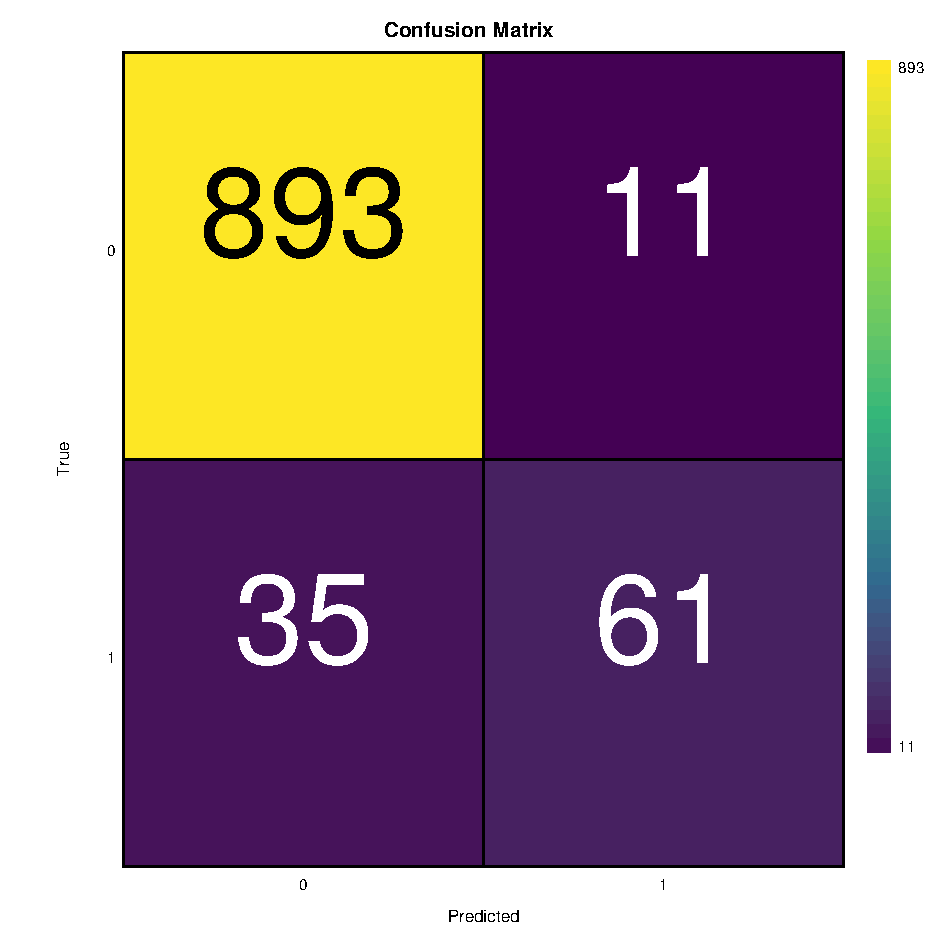
\includegraphics[width=\textwidth]{figures/confusion_matrix_lr}
    \caption{Confusion matrix}
\end{subfigure}
\hfill
\begin{subfigure}[b]{0.48\textwidth}
    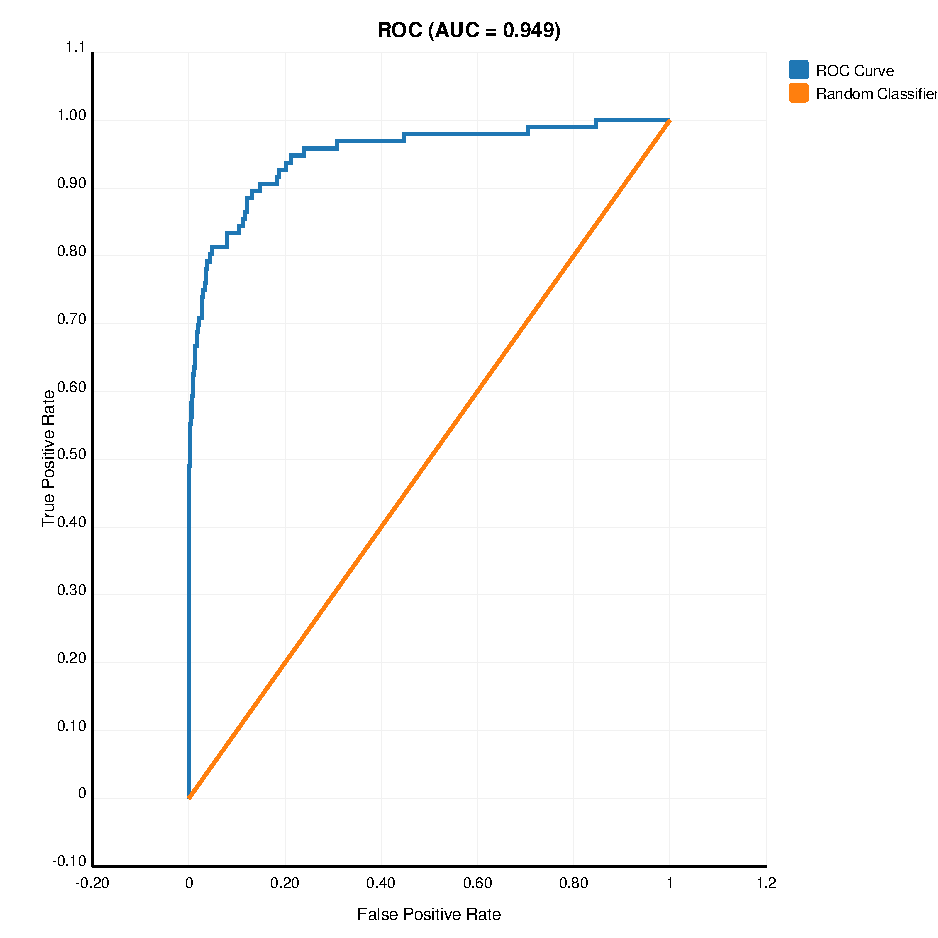
\includegraphics[width=\textwidth]{figures/roc_curve_lr}
    \caption{ROC curve (AUC = 0.9491)}
\end{subfigure}
\caption{Logistic Regression test-set performance. Recall on the minority class
         drops to 63.5\%, missing over a third of potential loan acceptors.}
\label{fig:lr_eval}
\end{figure}

The Random Forest improves minority-class recall by \textbf{+29.2 percentage
points} (92.7\% vs 63.5\%) and AUC by \textbf{+0.049} (0.998 vs 0.949) over
Logistic Regression, demonstrating the benefit of nonlinear ensemble methods on
this dataset.

% ──────────────────────────────────────────────────────────
\section{Practical Implications}
% ──────────────────────────────────────────────────────────

The predictive model developed in this study has direct implications for
Universal Bank's personal loan marketing strategy.

\subsection{Customer Targeting}

The Random Forest model and feature importance analysis identify three primary
customer segments with high loan acceptance probability:

\begin{enumerate}[leftmargin=*, itemsep=4pt]
    \item \textbf{High-income, high-spending customers:} Customers with annual
          income above \$100K and monthly credit card spending above \$3K show
          the strongest loan acceptance rates. These customers have both the
          financial capacity and spending behavior that correlate with loan
          interest.

    \item \textbf{Advanced-degree holders:} Customers with Education level 3
          (advanced/professional degree) are disproportionately represented
          among loan acceptors, particularly when combined with high income.

    \item \textbf{CD Account holders:} Customers with existing certificate of
          deposit accounts show elevated acceptance rates, suggesting that
          deeper banking relationships signal receptiveness to additional
          products.
\end{enumerate}

\subsection{Expected Campaign Improvement}

The previous blanket campaign achieved a 9.6\% acceptance rate across all
5{,}000 customers. By using the Random Forest model to target only predicted
acceptors:

\begin{itemize}[itemsep=2pt]
    \item \textbf{Precision of 97.8\%} means that nearly all customers flagged
          by the model will actually accept the loan, virtually eliminating
          wasted marketing contacts.
    \item \textbf{Recall of 92.7\%} means the model identifies the vast
          majority of potential acceptors---only about 7 out of every 96 true
          prospects would be missed.
    \item The bank can achieve comparable loan conversion with
          \textbf{approximately 10\% of the marketing effort}, dramatically
          improving cost efficiency.
\end{itemize}

\subsection{Deployment Considerations}

\begin{itemize}[itemsep=2pt]
    \item The model requires only 11 readily available customer attributes,
          all of which the bank already collects.
    \item Predictions can be generated in batch for campaign planning or in
          real-time for event-triggered offers.
    \item The probability threshold (default 0.5) can be adjusted: lowering it
          increases recall (captures more prospects) at the cost of more false
          positives, while raising it improves precision for high-confidence
          targeting.
\end{itemize}

% ──────────────────────────────────────────────────────────
\section{Conclusion and Recommendations}
% ──────────────────────────────────────────────────────────

This analysis demonstrates that machine learning can substantially improve
Universal Bank's personal loan campaign effectiveness. The key findings and
recommendations are:

\begin{enumerate}[leftmargin=*, itemsep=4pt]
    \item \textbf{Deploy the Random Forest model} as the primary targeting
          tool. With 99.1\% accuracy and 0.998 AUC, it provides highly reliable
          predictions using only standard customer data.

    \item \textbf{Prioritize three customer segments} for loan offers:
          high-income/high-spending customers, advanced-degree holders, and
          CD account holders. These segments, identified through both feature
          importance analysis and exploratory visualization, represent the
          highest-probability prospects.

    \item \textbf{Monitor model performance} over time, as customer behavior
          patterns may shift. Periodic retraining on updated campaign data is
          recommended to maintain accuracy.

    \item \textbf{Consider ensemble refinement:} Gradient Boosting achieved
          comparable CV accuracy (98.82\% vs 98.80\%) and may offer
          complementary strengths. An ensemble of both models could provide
          additional robustness.

    \item \textbf{Future enhancements:} Feature engineering (e.g.,
          Income/CCAvg ratio, interaction terms), hyperparameter optimization,
          and SHAP-based individual prediction explanations could further
          improve model performance and interpretability.
\end{enumerate}

\end{document}
